\clearpage
\VerdierPhysicalPageAnchor{0096}%
\begingroup
\setlength{\abovedisplayskip}{3pt plus 2pt minus 2pt}%
\setlength{\belowdisplayskip}{3pt plus 2pt minus 2pt}%
\VerdierSemanticAnchor{ch1-3-3-2-open-morphism-continuation}
これは $\operatorname{comp}(C)$ において
$u\colon X\to Y$ のホモトピー類に属するものとする。
\VerdierSemanticAnchor{ch1-3-3-2-representative}
すると $\operatorname{Tr}_1(C)$ の対象
$X\xrightarrow{\dot f}Y$ が得られる。
\VerdierSemanticAnchor{ch1-3-3-2-completion-cone}
完全三角
\begin{equation*}
  X\xrightarrow{u}Y\xrightarrow{\dot p(f)}c(f)
  \xrightarrow{\dot q(f)}X[1]
\end{equation*}
\VerdierSemanticAnchor{ch1-3-3-2-completion-conclusion}
は射 $u$ を含む。

\VerdierSemanticAnchor{ch1-3-3-3}
\noindent\textbf{命題 3.3.3. (TRII)}\quad
\VerdierSemanticAnchor{ch1-3-3-3-trii}
\textit{$K(C)$ の三角
$X\xrightarrow{u}Y\xrightarrow{v}Z\xrightarrow{w}X[1]$ が完全三角である
ための必要十分条件は、三角
$Y\xrightarrow{v}Z\xrightarrow{w}X[1]\xrightarrow{-u[1]}Y[1]$
が完全三角であることである。}

\VerdierSemanticAnchor{ch1-3-3-3-proof-forward}
三角 $X\xrightarrow{u}Y\xrightarrow{v}Z\xrightarrow{w}X[1]$ が
完全三角であると仮定する。このとき、これは次の形の三角に同型である：

\VerdierSemanticAnchor{ch1-3-3-3-cone-model}
\begin{equation*}
  X'\xrightarrow{\dot f}Y'\xrightarrow{\dot p(f)}c(f)
  \xrightarrow{\dot q(f)}X'[1],
\end{equation*}
ここで $X'\xrightarrow{\dot f}Y'$ は $\operatorname{Tr}_1(C)$ の対象である。
したがって、三角

\VerdierSemanticAnchor{ch1-3-3-3-rotated-model}
\begin{equation*}
  Y'\xrightarrow{\dot p(f)}c(f)\xrightarrow{\dot q(f)}X'[1]
  \xrightarrow{-\dot f[1]}Y'[1],
\end{equation*}
が完全三角であることを示せばよい。(3.2.6) により、図式

\VerdierSemanticAnchor{ch1-3-3-3-comparison}
\begin{center}
  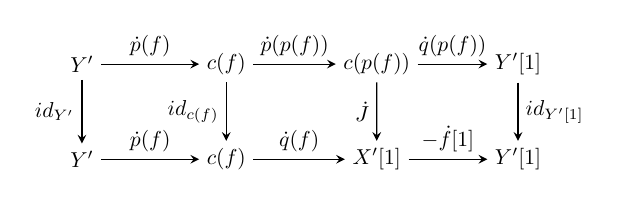
\begin{tikzpicture}[>=stealth,scale=0.78,every node/.style={transform shape}]
    \node (Y1)  at (0,1.55) {$Y'$};
    \node (Cf1) at (2.35,1.55) {$c(f)$};
    \node (Cpf) at (4.80,1.55) {$c(p(f))$};
    \node (Ys1) at (7.10,1.55) {$Y'[1]$};
    \node (Y2)  at (0,0) {$Y'$};
    \node (Cf2) at (2.35,0) {$c(f)$};
    \node (Xs)  at (4.80,0) {$X'[1]$};
    \node (Ys2) at (7.10,0) {$Y'[1]$};
    \draw[->] (Y1) -- node[above] {$\dot p(f)$} (Cf1);
    \draw[->] (Cf1) -- node[above] {$\dot p(p(f))$} (Cpf);
    \draw[->] (Cpf) -- node[above] {$\dot q(p(f))$} (Ys1);
    \draw[->] (Y2) -- node[above] {$\dot p(f)$} (Cf2);
    \draw[->] (Cf2) -- node[above] {$\dot q(f)$} (Xs);
    \draw[->] (Xs) -- node[above] {$-\dot f[1]$} (Ys2);
    \draw[->] (Y1) -- node[left] {$\operatorname{id}_{Y'}$} (Y2);
    \draw[->] (Cf1) -- node[left] {$\operatorname{id}_{c(f)}$} (Cf2);
    \draw[->] (Cpf) -- node[left] {$\dot J$} (Xs);
    \draw[->] (Ys1) -- node[right] {$\operatorname{id}_{Y'[1]}$} (Ys2);
  \end{tikzpicture}
\end{center}

\VerdierSemanticAnchor{ch1-3-3-3-forward-conclusion}
は $K(C)$ における三角の同型である。

\VerdierSemanticAnchor{ch1-3-3-3-proof-reverse}
次に、三角
$Y\xrightarrow{v}Z\xrightarrow{w}X[1]\xrightarrow{-u[1]}Y[1]$ が
完全三角であると仮定する。(3.2.4) から、三角

\VerdierSemanticAnchor{ch1-3-3-3-shifted-triangle}
\begin{equation*}
  Y[-1]\xrightarrow{v[-1]}Z[-1]\xrightarrow{w[-1]}X
  \xrightarrow{u}Y
\end{equation*}
は完全三角であり、さらに、
\VerdierSemanticAnchor{ch1-3-3-3-double-rotation}
先の議論を二度適用すれば、三角
\begin{equation*}
  X\xrightarrow{u}Y\xrightarrow{v}Z\xrightarrow{w}X[1]
\end{equation*}
\VerdierSemanticAnchor{ch1-3-3-3-conclusion}
も完全三角であることが従う。これで証明が完了する。
\endgroup

